% !TEX root = ./Basilisk-rwNullspace-20190209.tex


\begin{figure}[H]
	\centerline{
		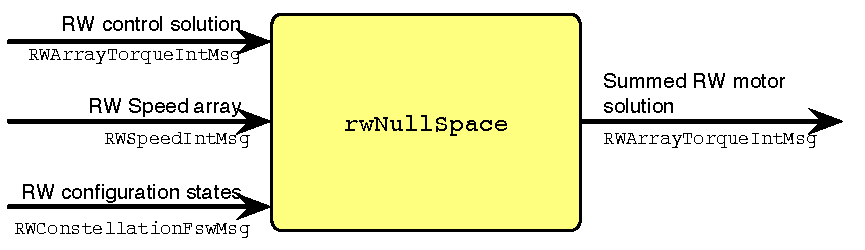
\includegraphics{Figures/moduleImg}
	}
	\caption{Module Input and Output Message Illustration.}
	\label{fig:moduleImg}
\end{figure}


\section{Module Description}
\subsection{Module Purpose}
This module aims to reduce the reaction wheel (RW) speeds by using the null space of the RW array.  The input and output messages of {\tt rwNullSpace} are shown in Figure~\ref{fig:moduleImg}.  There are three required input messages:
\begin{enumerate}
	\item The feedback control torque which is mapped onto the RW motor torque solution space.  The message type is {\tt RWArrayTorqueIntMsg}, the same message type as the module output message.
	\item The RW speed array message of type {\tt RWSpeedIntMsg}.
	\item The RW configuration message contains the RW spin axes information. The message type is {\tt RWConstellationFswMsg}.
\end{enumerate}
The module output message is a RW motor torque array message that sums the input control torque solution with the new null space torque solution that will reduce the RW speeds.  


\subsection{RW Null Space Mathematics}
Let $N$ be the number of RWs present, while $\hat{\bm g}_{s_{i}}$ is the $i^{\text{th}}$ RW spin axis unit direction vector.  The RW spin axes matrix is defined as
\begin{equation}
	[G_{s}] = [\hat{\bm g}_{s_{1}} \cdots \hat{\bm g}_{s_{N}}]
\end{equation}
The null motion RW projection matrix $[\tau]$ is given by\cite{schaub}
\begin{equation}
	[\tau] = [I_{N\times N}] - [G_{s}]^{T} \left( [G_{s}] [G_{s}]^{T} \right)^{-1} [G_{s}]
\end{equation}
This project matrix maps any vector $\bm d$ into the null-space of $[G_{s}]$ such that no torque is exerted onto the spacecraft.  As a result, these null-motion solution never impact the stability or performance of the RW attitude control solution.  This concept is illustrated through:
\begin{align*}
	[G_{s}] [\tau] &= [G_{s}] \left( [I_{N\times N}] - [G_{s}]^{T} \left( [G_{s}] [G_{s}]^{T} \right)^{-1} [G_{s}] \right)
	\\
	&= [G_{s}] - [G_{s}] [G_{s}]^{T} \left( [G_{s}] [G_{s}]^{T}] \right)^{-1} [G_{s}] \\
	&= [G_{s}] - [G_{s}] \\
	&= [0_{N\times N}]
\end{align*}


\subsection{RW Wheel Speed Reduction Control}
Let $J_{s_{i}}>0$ be the RW inertia about the spin axis $\hat{\bm g}_{s_{i}}$, $\Omega_{i}$ be the RW spin speed, and $\dot{\bm \omega}$ be the inertial spacecraft angular acceleration vector.  The RW motor torque equation is given by\cite{schaub}
\begin{equation}
	u_{s_{i}} = J_{s_{i}} (\dot\Omega_{i} + \hat{\bm g}_{s_{i}}^{T} \dot{\bm \omega} )
\end{equation}
Assuming that the spacecraft angular accelerations are much smaller than the wheel accelerations, this is approximated as
\begin{equation}
	u_{s_{i}} \approx J_{s_{i}} \dot\Omega_{i}
\end{equation}
Let $d_{i}$ be the desired torque to reduce the $i^{\text{th}}$ RW spin rate $\Omega_{i}$ given through
\begin{equation}
	d_{i} = - K \Omega_{i}
\end{equation}
where the feedback gain $K>0$.  Then setting $u_{s_{i}} = d_{i}$ ideally provides the stable closed loop response
\begin{equation}
	J_{s_{i}} \dot\Omega_{i} + K\Omega_{i} = 0
\end{equation}



Let $\bm d$ be the $N\times 1$ array of desired RW decelerating motor torques given by
\begin{equation}
	\bm d = -K \bm\Omega
\end{equation}
If this RW motor torque were directly applied then a non-zero torque would be produced onto the spacecraft causing attitude deviations.  Instead, this desired despin torque $\bm d$ is mapped through $[\tau]$ onto the null space of the RW array using
\begin{equation}
	\bm u_{s,\text{null}} = [\tau] \bm d
\end{equation}

Assume the attitude feedback RW motor control solution is given by $\bm u_{s,\text{cont}}$, then final module RW motor torque array is the sum of these two torques.
\begin{equation}
	\bm u_{s} = \bm u_{s,\text{cont}} + \bm u_{s,\text{null}} 
\end{equation}




